Child labour is a global phenomenon. Employment of children in any manual work is known as child labour. According to the Child labour (prohibition and regulation) act, 1986. A child is a person who has not yet attained the age of fourteen years. In this tender age where a child is expected to grow , enjoy its childhood to the fullest , seek condition, gain a strong value system goes to work to earn a living either for himself/herself and for their family. Child labour also deprives children of their dignity, potential and their childhood. Children working below the age of 14 years are not able to develop mentally, socially, physically and morally.

The organization of this Chapter is as follows. Section 1.1 describes Background of the project. Motivation of the project is represented in Section 1.2 Section 1.3 represents Problem statement of the project. Scope of the project is described in Section 1.4. Section 1.5 describes Objective of the project. Section 1.6 describes the selection of life cycle model. Section 1.7 shows the organization of report and finally, the Summary is described in 1.8 Section.

\section{Background}
Despite rates of child labour declining over the last few years, children are still being used in some severe forms of child labour such as bonded labour, child soldiers, and trafficking. Across India child labourers can be found in a variety of industries: in brick kilns, carpet weaving, garment making, domestic service, food and refreshment services (such as tea stalls), agriculture, fisheries and mining. Children are also at risk of various other forms of exploitation including sexual exploitation and production of child pornography, including online.

Not solving this problem can result in extreme bodily and mental harm, and even death of the victim. It can lead to slavery and sexual or economic exploitation. And in nearly every case, it cuts children off from schooling and health care, restricting their fundamental rights and threatening their futures.              


\section{Motivation}
Children on the move risk being forced into work or even trafficked – subjected to violence, abuse and other human rights violations. Children may be driven into work for various reasons. Most often, child labour occurs when families face financial challenges or uncertainty – whether due to poverty, sudden illness of a caregiver, or job loss of a primary wage earner. Hence,the project aims to reduce child labour and provide them with necessary resources so as the suffering children can lead a normal and peaceful life.

\section{Problem Definition}
Children are the future of nation and subjecting children to extreme labour causes bodily and mental harm of the child,which in long run threatens the future and development of the child and nation furthermore. Such crimes cannot be reduced unless they are brought in attention of the concerned authorities. To amend the situation of child labour, it is necessary for such crimes to come into attention. And to identify and then furthermore save the children from such labour,a system has to be developed.


\section{Scope}
The proposed system has a very minimal footprint on the overall system and can be easily accessed in the existing system. It will accept name, description and image of victim in a particular format, process and scrutinize it to check whether the activities involved fit into the specified occupations in The (Prohibition and Regulation) Child Labour Act,1986.\\ Following are the functions which this system is expected to do:
\begin{itemize}
\item The project will provide an efficient platform for the detection of child labour
\end{itemize}


\section{Objectives}
The proposed system is built to give a helping hand for prohibiting child labour and provide resources for regulating the lives of children who suffer.\\
The objectives of this project are as follows:
\begin{itemize}
\item To reveal the reasons and consequences of child labour.
\item To eradicate any kind of child abuse in the form of employment and prohibit maltreatment of children in workplace.
\end{itemize}


\section{Selection of Life cycle model for development}
The software development life cycle model selected for this project is the Waterfall Model. Waterfall approach was the first SDLC (Software Development Life Cycle) Model to be widely used in software engineering to ensure success of the project. It was developed by Winston W. Royce in 1970. In ”The Waterfall” approach, the whole process of software development is divided into separate phases, typically the outcome of one phase acts as the input for the next phase sequentially. All the phases are cascaded to each other in which progress is seen as flowing steadily downwards (like a waterfall) through the phases. Re-quirements for this project are well documented and fixed.

\begin{figure}[H]
    \centering
    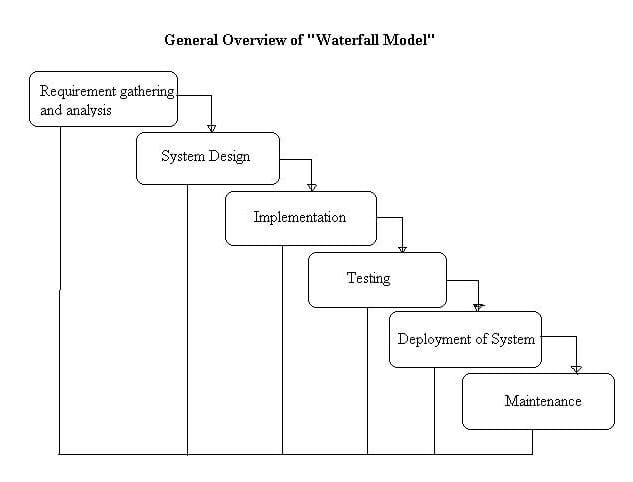
\includegraphics[scale=0.68]{introduction/Waterfall Model.jpg}
    \caption{ Waterfall Modell}
    \label{fig:my_label}
\end{figure}

Waterfall Model is best suited model for this project.
\begin{itemize}
\item Because requirements are easily understandable and defined
\item We can define requirements in early stage of development
\item User involvement in all phases is not necessary
\item Limited user’s participation
\end{itemize}
    
\section{Organization of Report}
\hspace{1cm}Chapter 1: entitled as Introduction describes the details about Background, Problem     Definition, Scope and Objective of the project, Identification of Software Development Process Model and Organization of report. \\

\hspace{0.5cm}Chapter 2: entitled as Project Planning and Management consists of details about the Feasibility Study, Risk Analysis, Project Scheduling, Effort Allocation and Cost Estimation of the project. \\

\hspace{0.5cm}Chapter 3: entitled as Analysis describes in detail, the Requirement Collection and Identification, H/w and S/w Requirements, Functional and Non-Functional Requirements and a Software Requirements Specification(SRS). \\

\hspace{0.5cm}Chapter 4: includes design about System Architecture, Data Flow Diagram and various UML Diagrams. \\
 


\section{Summary}
As mentioned in above sections, this project aims at building an ebuddy for rescuing child labour. The scopes, objective, etc. are as mentioned above. In the next chapter, project planning and management will be discussed.